The entry vehicle is required to perform the functions listed in the \gls{fbs} of Figure \ref{fig:fbs}, which categorises the main vehicle functions. These functions can subsequently be attributed to the subsystems partaking in the mission.

\begin{figure}[h]
	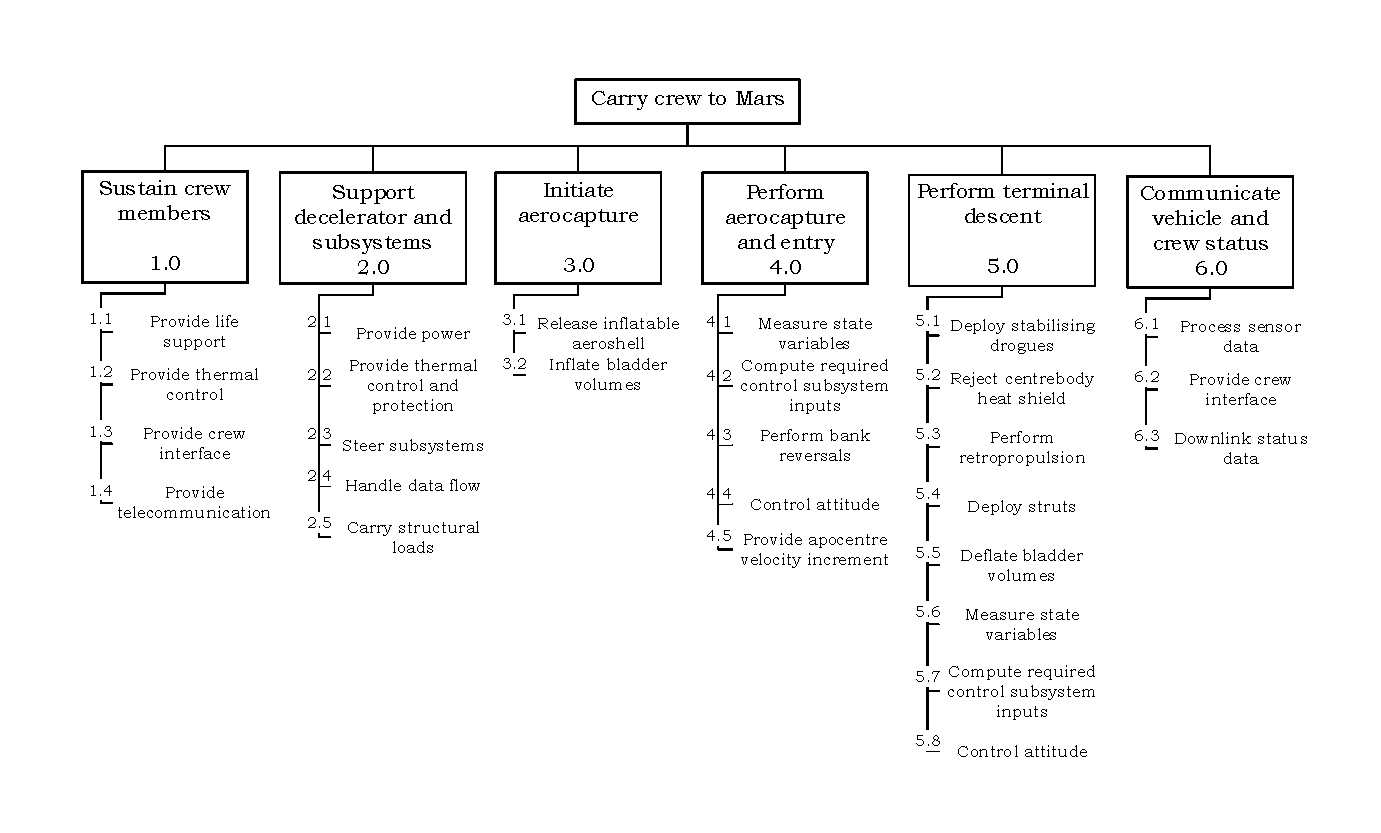
\includegraphics[width=0.95\textwidth]{./Figure/subsystem_breakdown/FBS.pdf}
	\caption{Entry vehicle \acrlong{fbs}}
	\label{fig:fbs}
\end{figure}

Sequencing the functions of the \gls{fbs} in time yields the \gls{ffd} in Figure \ref{fig:ffd}. Sequencing of sub-functions 3.1-3.2, 4.0-4.5 and 5.0-5.8 is taken up in the respective sections discussing their design. Sub-functions 1.1-1.4, 2.1-1.5 and 6.1-6.3 are performed continuously.

\begin{figure}[H]
	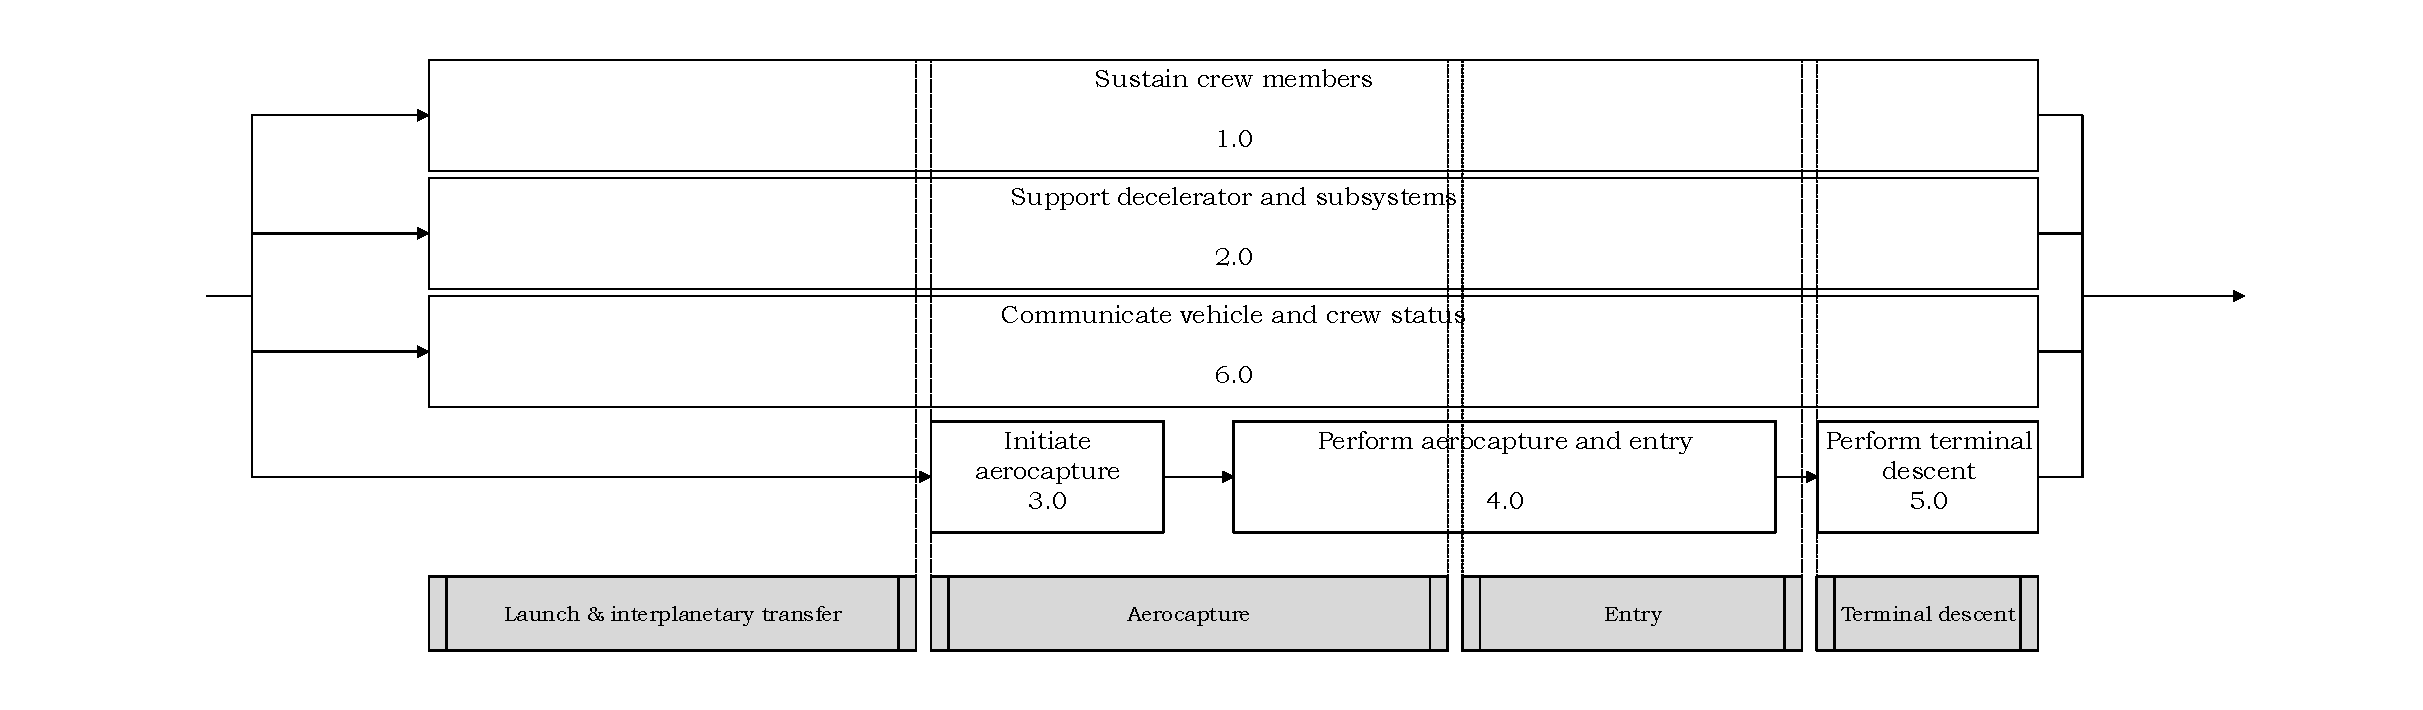
\includegraphics[width=1.00\textwidth]{./Figure/subsystem_breakdown/FFD.pdf}
	\caption{Entry vehicle \acrlong{ffd}}
	\label{fig:ffd}
\end{figure}



